The distributed algorithms are compared using the total number of backlogged packets after each \ac{SCA} update. \review{Fig. \ref{fig-d} compares the performances of the algorithms with the \ac{PL} varies uniformly between \me{[0,-6]} dB}. Each \ac{BS} serves \me{|\mc{U}_b| = 4} users in a coordinated manner to reduce the number of backlogged packets, whith the queued packets for each user is given by \me{Q_k = [5,7,9,11,8,12,5,4]} bits. As discussed in Section \ref{sec-4}, the performance and the convergence speed of the distributed algorithms are susceptible to the step size used in the subgradient update. Due to the fixed interference levels in the primal approach, it may lead to infeasible solutions if the initial or any intermediate update is not feasible.

Fig. \ref{fig-d} compares the primal and the \ac{ADMM} solutions for the \ac{JSFRA} scheme using the \ac{SCA} and by \ac{MSE} relaxation using the number of backlogged packets. In between the \ac{SCA} updates, the primal or the \ac{ADMM} scheme is performed for \me{J_{\max} = 20} iterations to exchange the respective coupling variables. The number of backlogged packets only at the \ac{SCA} points are marked in the figure. The performance of the distributed approaches are similar to the centralized schemes if the primal and dual updates are performed until convergence.
%In Fig. \ref{fig-d}, the total number of backlogged packets at each \ac{SCA} points are plotted without the inner loop iterations of \me{J_{\max}} times for the primal or the dual variables convergence. %It can be seen from Fig. \ref{fig-d} that the distributed algorithms approach the centralized scheme by exchanging minimal information between the coordinating \acp{BS}.
\begin{figure}
	\centering
	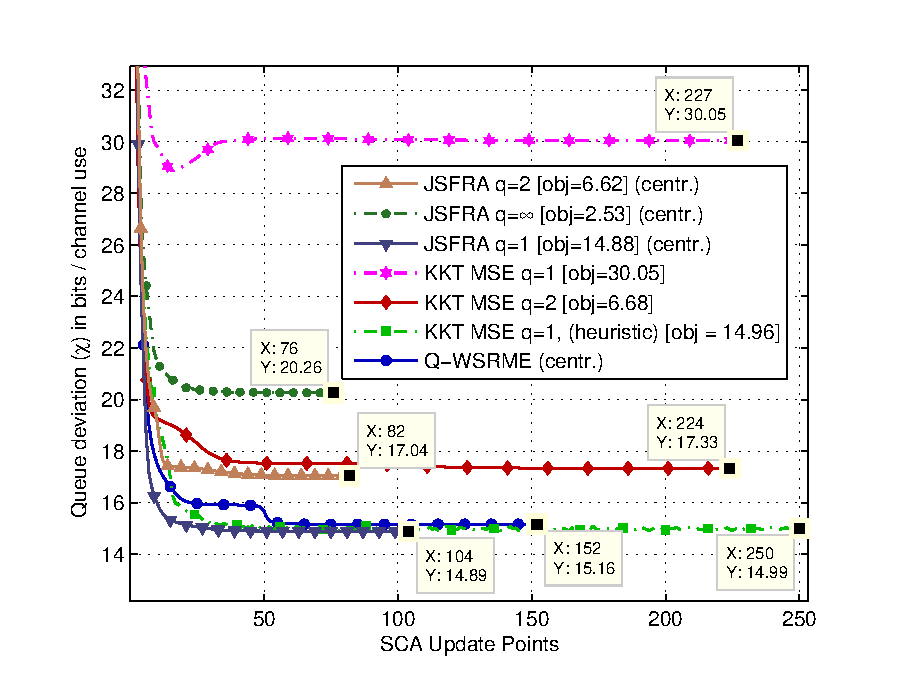
\includegraphics[width=\columnwidth]{fig-9-3}
	\caption{Impact of varying \me{q} in the total number of backlogged packets after each \ac{SCA} update for a system \me{\lbrace N,N_B,K,N_T,N_R \rbrace = \lbrace 5,2,8,4,1 \rbrace}}
	\label{fig-d-3.1}
\end{figure}

\review{Fig. \ref{fig-d-3.1} compares the performances of the centralized and the \ac{KKT} algorithm in Section \ref{sec-4.3} for different exponents with \me{Q_k = [9,16,14,16,9,13,11,12]} bits and the \ac{PL} varies uniformly between \me{[0,-3]} dB}. The \me{\ell_1} norm \ac{JSFRA} scheme performs better over other schemes due to the greedy objective. The \ac{KKT} approach for \me{\ell_1} norm is not defined due to the non-differentiability of the objective as discussed in the Section \ref{sec-4.3}. If used for \me{\ell_1} norm, the problem of over-allocation will not affect the dual variables \me{\sigma_{l,k,n}} and \me{\alpha_{l,k,n}} since the queue deviation is raised to the power zero in \eqref{kkt-mse-4.2}. A heuristic method based on subdifferential calculus in \cite{bertsekas1999nonlinear} is proposed in Fig. \ref{fig-d-3.1} by assigning zero for \me{\sigma_{l,k,n}} when \me{Q_k - t_k < 0}. It addresses the over-allocation in the \me{\ell_1} norm for dropping the absolute value operator from the objective. It can be seen that the heuristic method oscillates near the converging point with the deviation determined by the factor \me{\rho} used in \eqref{kkt-mse-4.1}. The objective values are mentioned in the legend for all the schemes and the objective of the \me{\ell_2} norm is not the same as that of the \me{\ell_1} norm used for plotting.
\begin{figure*}
	\centering
	\subfloat[][Average backlogged packets in the system after \me{250} transmission instants]{
		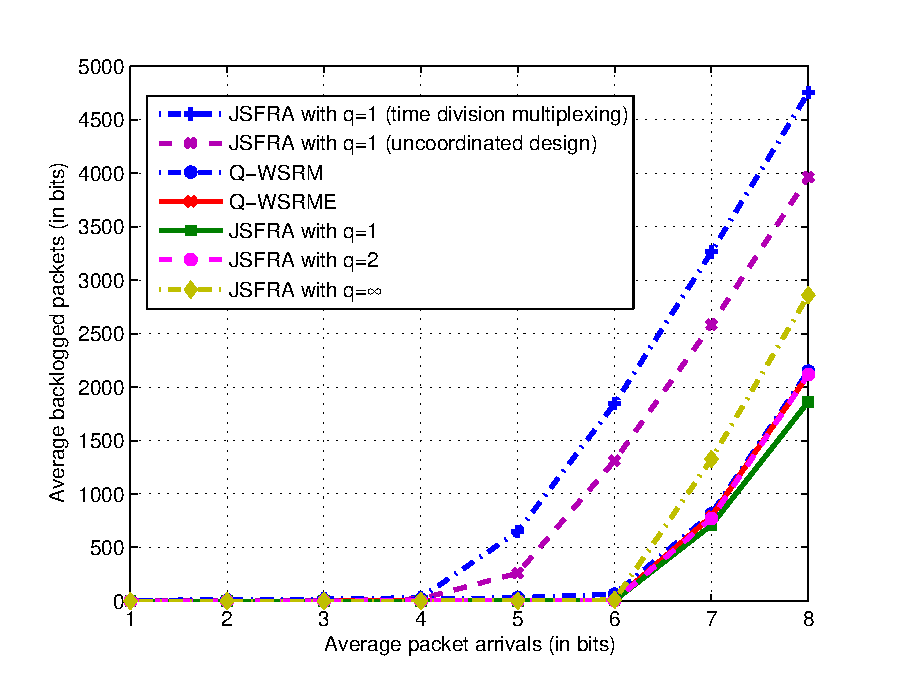
\includegraphics[width=0.48\textwidth]{average_queue_over_time-2}
		\label{fig-review}
	}
	\hfill
	\subfloat[][Total backlogged packets at each transmission slot for \me{A_k = 6} bits]{
		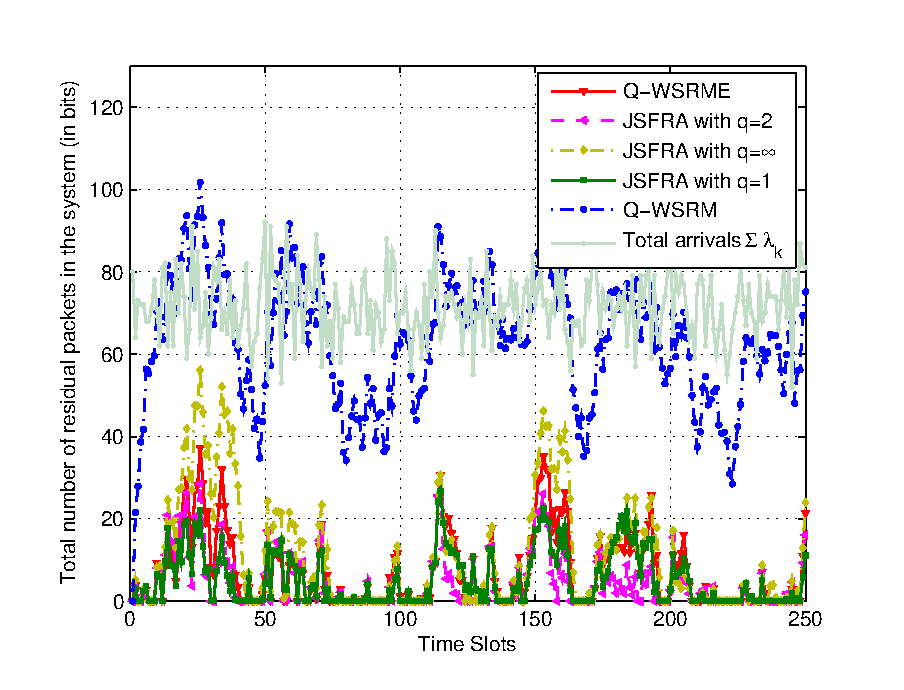
\includegraphics[width=0.48\textwidth]{instant_queue_over_time-2}
		\label{fig-review-time}
	}
	\caption{Time analysis of the Queue dynamics for a system \me{\lbrace N,N_B,K,N_T,N_R \rbrace = \lbrace 4,2,12,4,1 \rbrace}}
	\label{fig-time-analysis}
\end{figure*}
%The \me{\ell_2} norm for the \ac{JSFRA} and the \ac{KKT} approach achieves nearly the same value of \me{6.62} with different \me{\chi}, due to the limited number of iterations for the dual variable convergence between each \ac{SCA} update. Fig. \ref{fig-d-3.1} also shows the effect of dropping the squared rate variable from the objective in the \ac{Q-WSRME} scheme compared to the \me{\ell_2} norm which includes it. By dropping it, the \ac{Q-WSRME} scheme minimizes the number of queued packets in a prioritized manner based on the respective queues. On contrary, the \me{\ell_2} norm allocate rates to the users with the higher number of queued packets before addressing the users with the smaller number of queued packets.

\begin{comment}

In Fig. \ref{fig-d-2}, the performance of the distributed algorithms are studied for \me{K = 12} users utilizing \me{N = 6} sub-channels. The system considers \me{N_B = 3} \acp{BS}, each having \me{N_T = 4} transmit antennas serving \me{|\mc{U}_b| = 4} users equipped with \me{N_R = 2} antennas respectively. The users are assumed to have the path loss following the uniform distribution between \me{[0,-6]} dB from all \acp{BS}. The performance of the algorithms are similar to the \me{N_B = 2} \ac{BS} scenario discussed earlier.

Fig. \ref{fig-d-2} plots the performance of the centralized and the distributed algorithms at each \ac{SCA} update. In case of the distributed approaches, in between each \ac{SCA} update, the primal or the \ac{ADMM} exchanges are performed for \me{J_{\max} = 20} iterations. In practice, \me{J_{\max} = 1} can be set to perform the \ac{SCA} update, \ac{ADMM} or primal update, and the receive beamformers \me{\mvec{W}{k,n}} update at the same instant, which affects the convergence rate and the stationary point of the final solution. The data tips are used to highlight the convergent points of various algorithms. The performance of the \ac{JSFRA} schemes using the primal decomposition are notably inferior compared to the \ac{ADMM} approach for the same schemes. It is mainly attributed to the difficulty in selecting the step size for the system employing \me{N_B \geq 3} \acp{BS}.
\begin{figure*}[t]
	\centering
	\subfloat[][System \me{\lbrace N,N_B,K,N_R \rbrace = \lbrace 3,2,8,1 \rbrace}]{
		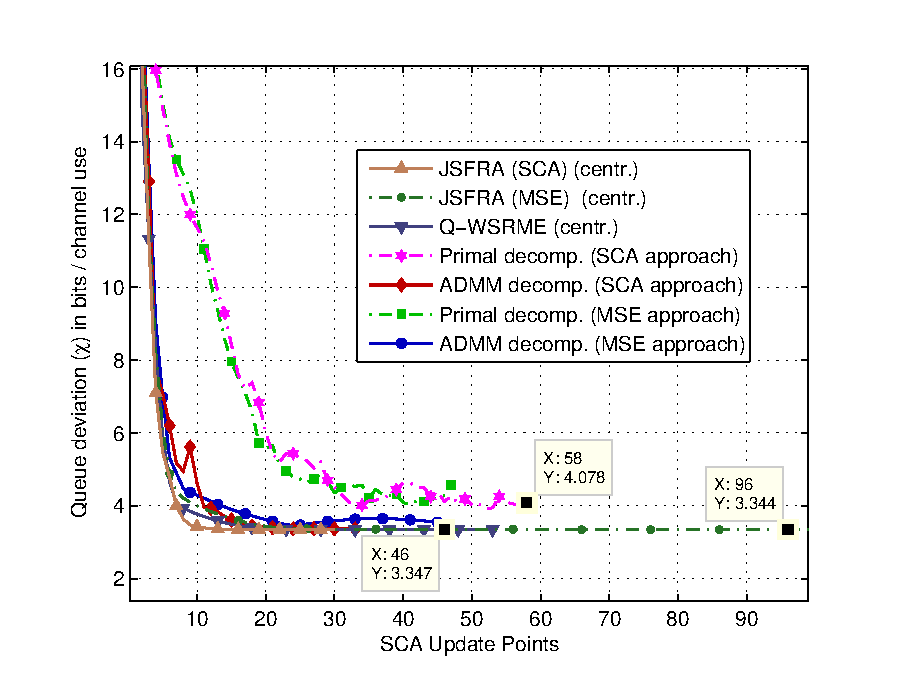
\includegraphics[width=0.48\textwidth]{fig-3-2}
		\label{fig-d-1}
	}
	\hfill
	\subfloat[][System \me{\lbrace N,N_B,K,N_R \rbrace = \lbrace 6,3,12,2 \rbrace}]{
		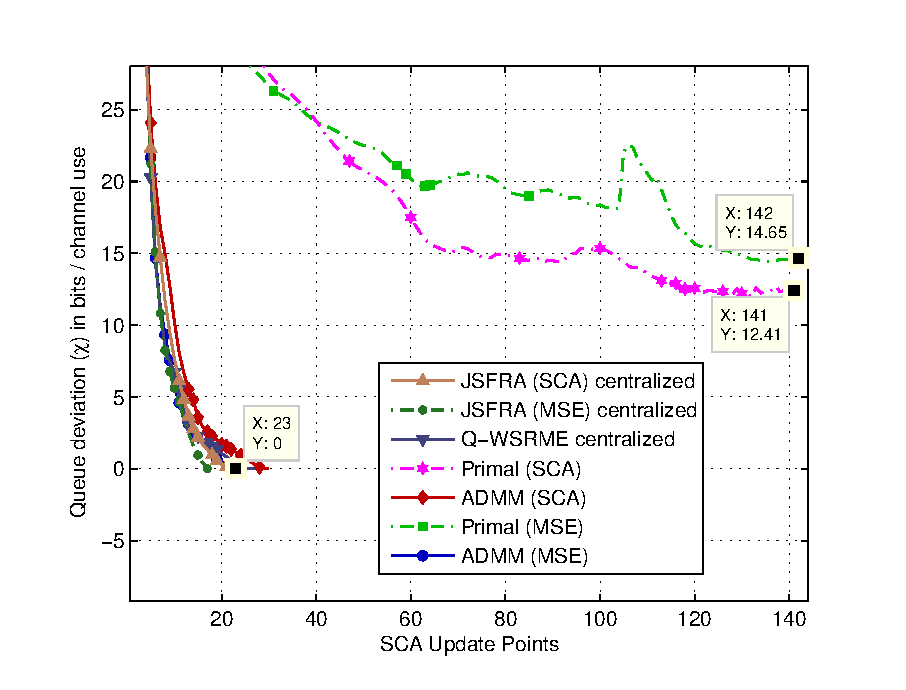
\includegraphics[width=0.48\textwidth]{fig-5-1}
		\label{fig-d-2}
	}
	\caption{Number of backlogged packets at each \ac{SCA} points}
	\label{fig-d}
\end{figure*}

\end{comment}